\documentclass[10pt,a4paper,openany,twoside,prof]{book}

\usepackage{layout_cours}
\usepackage{hyperref}

\setlist{leftmargin=5mm}

\begin{document}
	\chapnumber{1} % numéro du chapitre
	\titre{Ensembles de nombres} % titre du chapitre
	\classe{Seconde} % classe
	\entetegal

	% Debut du texte
	% **************
	\vspace{-7mm}
	\paragraph*{Objectif du chapitre:}
	\begin{itemize}  
		\vspace{-2mm}
		\setlength\itemsep{-1mm}
		\item Connaître et comprendre les ensembles de nombres $\N$, $\Z$, $\D$, $\Q$, $\R$.
	\end{itemize}
	\vspace{-7mm}

	
\section{Les entiers naturels: $\N$}
\begin{defi}{Entier naturel}{}
 Les \bf{entiers naturels} se construisent à partir de zéro et en ajoutant un pour obtenir le nombre suivant.

 On note $\N$ l'ensemble de ces nombres. Donc $$\mathbb{N}=\{ 0,\ 1,\ 2,\ 3,\ \dots \}$$
\end{defi}

\begin{rems}{}{}
La notation $\mathbb{N}$ représente la première lettre de \guillemotleft naturel\guillemotright.
\end{rems}

\section{Les entiers relatifs: $\Z$}
\begin{defi}{Entier relatif}{}
 Les \bf{entiers relatifs} se construisent à partir de zéro et en ajoutant un ou en retirant un pour obtenir le nombre suivant.

 On note $\Z$ l'ensemble de ces nombres. Donc $$\mathbb{Z}=\{ \dots ,\ -3,\ -2,\ -1,\ 0,\ 1,\ 2,\ 3,\ \dots \}$$
\end{defi}

\begin{rem}
	\begin{itemize}
		\item 
		La notation $\Z$ provient de la première lettre de \guillemotleft \textit{Zahlen}\guillemotright \ qui signifie nombres en allemand.
		\item Ce sont des nombres positifs. On dit que zéro est l'élément neutre.
	\end{itemize}
\end{rem}

\begin{prop}{}{}
	On a $\N\subset\Z$, c'est-à-dire que l'ensemble des entiers naturel est inclus dans l'ensemble des entiers relatifs.

	Plus précisément, on peut construire les entiers relatifs en prenant les entiers naturels et leurs opposés.
\end{prop}


\section{Les nombres réels: $\mathbb{R}$}

\vspace{-3mm}
\begin{defi}{Nombre réel}{}
	\begin{center}
		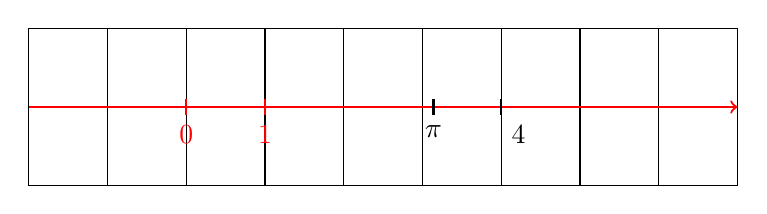
\begin{tikzpicture}
	\draw (-2,-1) grid (7,1);
	\draw[->, red, thick] (-2,0) -- (7,0);
	\draw[red, thick] (0, 0.1) -- (0, -0.1) node [below] {0};
	\draw[red, thick] (1, 0.1) -- (1, -0.1) node [below] {1};
	\draw[thick] (3.14, 0.1) -- (3.14, -0.1) node [below] {$\pi$};
	\draw[thick] (4, 0.1) -- (4, -0.1) node [below right] {$4$};
		\end{tikzpicture}
	\end{center}
	On considère une droite graduée et orientée vers la droite appelée \bf{droite réelle}. A chaque point de cette droite correspond un nombre. Ce nombre est la distance à l'origine avec un signe. Les positifs se situent à droite de l'origine et les négatifs à gauche.
	
	Un tel nombre est appelé \bf{nombre réel}. L'ensemble de ces nombres est noté $\R$.
\end{defi}

\begin{rem}{}{}
	C'est le plus grand ensemble de nombres que nous manipulerons cette année.
\end{rem}

\section{Les nombres rationnels: $\mathbb{Q}$}

\begin{defi}{Nombre rationnel}{}
Un nombre rationnel est un nombre qui peut s'écrire sous forme de fraction $\frac{a}{b}$ avec $a\in\Z$ et $b\in\N^*$ des entiers. 

 L'ensemble de tous les nombres rationnels est noté: $\mathbb{Q}$.
\end{defi}

\begin{ex}{}{}
\begin{itemize}
	\item $5/7$ est rationnel. Il est déjà sous forme d'une fraction
	\item $0.75 = 3/4$
	\item  $0,333\dots$ est rationnel, en effet c'est l'écriture décimale de la fraction $\dfrac{1}{3}$
\end{itemize}
\end{ex}

\begin{props}{}{}
	\begin{minipage}{0.4 \linewidth}
	\begin{center}
		\begin{itemize}
			\item $\sqrt{2}$ n'est pas rationnel. 
			
			Autrement dit, $\sqrt{2}\notin\Q$.

			\item $\pi\notin\Q$
		\end{itemize}
	\end{center}
	\end{minipage}
	\begin{minipage}{0.4 \linewidth}
	\begin{center}
		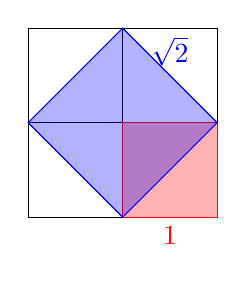
\begin{tikzpicture}[scale=1.2]
            \draw (-1,1) grid (1,3);
			\draw [fill, red, fill opacity = 0.3] (0,1)-- node[below, opacity =1] {1} (1,1) --(1,2) --  (0,2) -- (0,1);
			\draw [fill, blue, fill opacity = 0.3] (1,2)-- node[above, opacity =1] {$\sqrt{2}$} (0,3)  -- (-1,2) --  (0,1) --  (1,2);
		\end{tikzpicture}
	\end{center}
	\end{minipage}
\end{props}


% \begin{deme}{}{}
% 	On raisonne par l'absurde, en supposant que $\sqrt{2}\notin\Q$ (c'est-à-dire qu'il est rationnel). On va montrer que cela conduit à une contradiction de logique.

% 	Il existe $a\in\Z$ et $b\in\N^*$ des entiers tels que $\sqrt{2} = \frac{a}{b}$ et que la fraction est irréductible. Alors on a $2 = \frac{a^2}{b^2}$. Donc $a^2=2\times b^2$. Donc $a^2$ est pair. Alors $a$ aussi est pair.

% 	On écrit donc $a=2\times k$ avec $k\in\Z$. L'égalité $a^2=2b^2$ devient $4k^2 = 2b^2$. On obtient $2k^2=b^2$. Par le même raisonnement on en déduit que $b$ est pair.

% 	Alors la fraction $\frac{a}{b}$ se simplifie par $2$ et elle n'est pas irréductible. C'est absurde. L'hypothèse initiale est fausse et $\sqrt{2}$ n'est pas rationnel.
% \end{deme}


\begin{rems}{}{}
	\begin{itemize}
		\item 
		On ne peut donc pas écrire $\pi$ comme une fraction. En revanche, on peut trouver des fractions proches (et même aussi proche que l'on veut). Par exemple $\frac{22}{7} \approx 3.143$.
		\item Attention, toutes les racines ne sont pas irrationnelles. Par exemple, $\sqrt{36}=6\in\Q$. On a même $\sqrt{6}\in\N$.
	\end{itemize}
\end{rems}


\begin{rem}{}{}
	
On fera attention aux règles de calcul :


\begin{minipage}{7cm}
\begin{center}
 addition (réduire au même dénominateur)
\end{center} \[  \frac{a}{b}+\frac{x}{y}=\frac{ay+xb}{by} \] \end{minipage}
\vline
\begin{minipage}{5cm}
\begin{center}
 multiplication
 \end{center} \[  \frac{a}{b}\times \frac{x}{y}=\frac{a \times x}{b \times y} \] 
\end{minipage}
\vline
\begin{minipage}{4cm}
\begin{center}
division
\end{center}\[  \frac{ \frac{a}{b} }{ \frac{x}{y}}=\frac{a}{b}\times \frac{y}{x}. \] 
\end{minipage}

\medskip
Rappelons encore que pour simplifier une fraction il faut qu'il y ait un facteur \\commun au numérateur et au dénominateur: \[  \frac{a\times {\color{orange}x}}{b\times {\color{orange}x}}=\frac{a}{b} \]

\medskip
Une astuce d'écriture qui nous sera souvent utile \[ \frac{a}{b}=\frac{1}{b}\times a \]
\end{rem}

\begin{prop}{Priorité de calcul}{}
 Pour effectuer un calcul on respectera l'ordre de priorité :
\begin{enumerate}
\item Les calculs entre parenthèses ou crochets. S'il y a des parenthèses emboîtées les plus emboîtées sont prioritaires. La barre de fraction joue le même rôle que des parenthèses autour des numérateurs et dénominateurs.
\item Les exposants (puissances)
\item Les multiplications et division.
\item Les additions et soustractions.
\end{enumerate}
\end{prop}

\begin{histoire}{}{}
	Nous sommes au IIIe siècle av J.C. dans la fameuse école de géométrie créée par Pythagore lui-même. Ses disciples tentent d'approcher la diagonale d'un carré de côté 1 avec par un rapport, c'est-à-dire une fraction. Or cette diagonale mesure $\sqrt{2}$. Les élèves se rendent compte qu'une valeur approchée ne convient pas à la formule du théorème de Pythagore.
	La géométrie atteint ses limites, il faut désormais penser des nombres qui ne se lisent pas sur les figures.

	C'est un véritable coup de tonnerre. L'école pythagoricienne avait en effet pour ambition de montrer que l'univers géométrique pouvait entièrement se comprendre avec des nombres rationnels, c'est-à-dire des fraction. Ils décident de garder le secret.
	
	Finalement, un des membres de la Fraternité, Hippase de Métaponte, trahit le secret et révèle au monde l'existence de nombres irrationnels.

L'historien et philosophe, Proclus (Ve siècle), déclara à ce sujet :
« On dit que les gens qui ont divulgué les nombres irrationnels ont péri dans un naufrage jusqu'au dernier, car l'inexprimable, l'informe, doit être absolument tenu secret ; ceux qui l'ont divulgué et ont touché à cette image de la vie ont instantanément péri et doivent rester éternellement ballottés par les vagues. »


Euclide d'Alexandrie (-320 ; -260) présente une des premières démonstrations de l'irrationalité de $\sqrt{2}$.

\end{histoire}

\begin{defi}{Fraction irréductible}{}
	Lorsqu'il n'est pas possible de simplifier davantage une fraction, on dit qu'elle est \bf{irréductible}. On préférera toujours cette écriture lorsque c'est possible.
\end{defi}

\begin{ex}{}{}
	$\frac{35}{21} = \frac{5}{3}$

	$\frac{102}{132} = \frac{17}{22}$
\end{ex}

\section{Les nombres décimaux: $\mathbb{D}$}

\begin{defi}{Nombre décimal}{}
	Si un nombre réel $x\in\R$ admet une admet un développement décimal limité, c'est-à-dire s'il possède une \bf{écriture décimale} avec un nombre fini de chiffres après la virgule, alors on dit que c'est un \bf{nombre décimal}.

 L'ensemble des nombres décimaux est noté $\mathbb{D}$. 
\end{defi}

\begin{ex}{}{}
	\begin{itemize}
		\item $3.14$ est un nombre décimal. Mais $\pi$ n'est en pas un.
		\item $4/5 = 0.8$ est un nombre décimal
	\end{itemize}
\end{ex}

\begin{prop}{}{}
	On a $\D\subset\Q$, c'est-à-dire que tous les nombres décimaux sont des nombres rationnels.
\end{prop}

\begin{dem}{}{}
	On se donne un nombre décimal $x\in\D$. Il existe des chiffres $a_1, a_2, \cdots , a_n$ et $b_1, b_2, \cdots, b_m$ entre 0 et 9 tels que $x=\overline{a_1 a_2 \cdots a_n , b_1 b_2 \cdots b_m}$

	On multiplie alors par 10 autant de fois qu'il est nécessaire, ici m fois, pour obtenir un entier au numérateur.

	$x = \frac{\overline{a_1 a_2 \cdots a_n b_1 b_2 \cdots b_m}}{10^m}$

	Donc $x$ s'écrit comme une fraction et $x\in\Q$
\end{dem}

\begin{ex}{}{}
	$0.45 = \frac{45}{100} = \frac{9}{20}$
	
	$45.7554 = \frac{457554}{10000}$
\end{ex}

\begin{notation}{}{}
	Lorsque l'écriture décimale a une infinité de chiffres qui se répète, on utilise une barre au dessus de la séquence qui se répète.
\end{notation}

\begin{ex}{}{}
	\begin{itemize}
		\item 
		$1/3 = 0.3333\ldots = 0.\overline{3}$
		\item $\frac{2}{11} = 0.181818\ldots = 0.\overline{18}$
		\item $\frac{1}{7} = 0,142857142857\ldots = 0,\overline{142857}$
	\end{itemize}
\end{ex}

\begin{rem}{}{}
	On remarque que le développement décimal d'une fraction est périodique (il y a un motif qui se répète). On peut le voir en effectuant la division euclidienne. A chaque étape, il y a un nombre fini de reste possibles. Dès que l'on trouve un reste déjà obtenu, alors on entame un motif identique au précédente.
\end{rem}

\begin{prop}{}{}
	$\frac{1}{3}\notin\D$, c'est-à-dire que $\frac{1}{3}$ n'est pas un nombre décimal.
\end{prop}

\begin{deme}{}{}
	On va raisonner par l'absurde. Supposons que $\dfrac{1}{3}$ soit décimal. Alors il est de la forme $\dfrac{a}{10^n}$ avec $a\in\Z$ et $n\in\N$.

On a donc $\dfrac{1}{3} = \dfrac{a}{10^n}$.

Doù, $10^n = 3 \times a$

A gauche, d'après le critère de divisibilité par 3, $10^n$ n'est pas divisibile par 3.
Tandis qu'à droite on a un multiple de 3. 

 On obtient une contradiction. Donc $\dfrac{1}{3}$ n'est pas décimal.
\end{deme}


\begin{defi}{Ecriture scientifique}{}
	L'\textbf{écriture scientifique} est l'écriture sous forme du produit d'un nombre décimal ayant un seul chiffre non nul avant la virgule et d'une puissance de 10 (d'exposant entier relatif).
\end{defi}

\begin{ex}{}{}
	$38 = 3,8 \times 10^1$ \hspace{0.8cm} ou \hspace{0.8cm} $0,0562 = 5,62 \times 10^{-2}$ \hspace{0.8cm}ou  encore \hspace{0.8cm} $-97631 = - 9,7631 \times 10^{4}$
\end{ex}

\begin{methode}{Trouver un encadrement à $10^{-n}$ près}{}
	On se donne un réel $x\in\R$, par exemple $x=\pi$. On veut en trouver un encadrement à $10^{-n}$ près, avec par exemple $n=6$. La tolérance est donc de $0,000001$.
	On veut donc trouver deux réels $a<b$ tels que $a$ et $b$ soient proches à $0,000001$ près et $a\le x\le b$.

	\begin{enumerate}
		\item 
		Avec la calculatrice on trouve une approximation de $x$ avec $n+1$ chiffres après la virgule: 
		$\pi\approx 3.1415926$
		\item 
		On choisit les deux bornes $a = 3.141592$ et $b=3.141593$, en conservant les $n$ premiers chiffres.
		\item 
		On a bien $3.141592\le \pi \le 3.141593$. et $b-a=0,000001$.
	\end{enumerate}


\end{methode}

\begin{rem}{}{}
	Attention à ne pas prendre seulement $n$ chiffres. Dans l'exemple ci-dessus, on aurait conclu que $\pi\approx 3.141593$ et on aurait tenté de dire que $3.141593\le \pi \le 3.141594$, ce qui est faux !	
\end{rem}

\section{Schéma bilan}
\vspace{1cm}
	\begin{minipage}{0.4 \linewidth}
	\begin{center}
	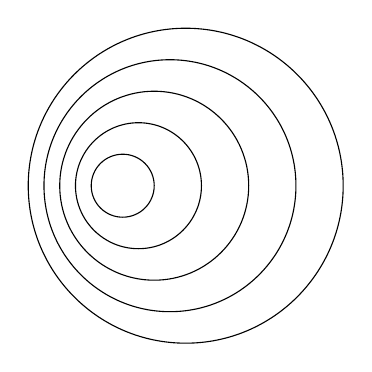
\begin{tikzpicture}[scale=0.4]
		\draw (0.5,0) circle (1);
		\node at (0.5,0) {$\N$};
		\draw (1,0) circle (2);
		\node at (2,0) {$\Z$};
		\draw (1.5,0) circle (3);
		\node at (3.5,0) {$\D$};    
		\draw (2,0) circle (4);
		\node at (5,0) {$\Q$};
		\draw (2.5,0) circle (5);    
		\node at (7,0) {$\R$};
	\end{tikzpicture}
	\end{center}
	\end{minipage}
	\begin{minipage}{0.4 \linewidth}
		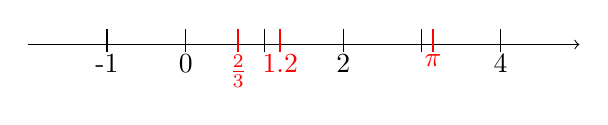
\begin{tikzpicture}[scale=1]
		\draw[->] (-2,0) -- (5,0);
		\draw (-1, -0.1) -- (-1, 0.2);
		\draw (0, -0.1) -- (0, 0.2);
		\draw (1, -0.1) -- (1, 0.2);
		\draw (2, -0.1) -- (2, 0.2);
		\draw (3, -0.1) -- (3, 0.2);
		\draw (4, -0.1) -- (4, 0.2);
		\draw[red, thick] (1.2, -0.1) -- (1.2, 0.2);
		\draw[red, thick] (3.14, -0.1) -- (3.14, 0.2);
		\draw[red, thick] (0.666, -0.1) -- (0.666, 0.2);
		\node [below] at (-1,0) {-1};
		\node [below] at (4,0) {4};
		\node [below] at (2,0) {2};
		\node [below] at (0,0) {0};
		\node [below, red, thick] at (3.14,0) {$\pi$};
		\node [below, red, thick] at (1.2,0) {$1.2$};
		\node [below, red, thick] at (0.666,0) {$\frac{2}{3}$};
	\end{tikzpicture}
	\end{minipage}

\newpage
\section{Exercices}
\sectionexo{Calcul avec les fractions}
37,38,39 p.100

\sectionexo{Nombres rationnels, décimaux}
35, 36, 38 p.65
120 p.69


\sectionexo{Approximation décimale}
114 p.69
115, 116 p.69

\end{document}


% \begin{prop}{}{}
% Lorsqu'un nombre a une écriture décimale infinie périodique c'est un nombre rationnel.
% \end{prop}

% \begin{rem}{}{}
% On dit que l'écriture est périodique lorsqu'une série de chiffre se reproduit indéfiniment.
% \end{rem}


